\documentclass[conference]{IEEEtran}
\IEEEoverridecommandlockouts
% The preceding line is only needed to identify funding in the first footnote. If that is unneeded, please comment it out.
\usepackage{cite}
\usepackage{amsmath,amssymb,amsfonts}
\usepackage{tikz}
\usetikzlibrary{arrows.meta, positioning}
\usepackage{hyperref}
\usepackage{algorithmic}
\usepackage{graphicx}
\usepackage{textcomp}
\usepackage{xcolor}
\usepackage{xurl}
\def\BibTeX{{\rm B\kern-.05em{\sc i\kern-.025em b}\kern-.08em
    T\kern-.1667em\lower.7ex\hbox{E}\kern-.125emX}}
\begin{document}

\title{ Kernel - Level Semantic Search with Knowledge Graphs
}

% \author{\IEEEauthorblockN{\textsuperscript}
% \and
% \IEEEauthorblockN{Arjun Deodhar}

% \IEEEauthorblockA{\textit{COEP Technological University} \\
% Dept. of Computer Science\\
% % \textit{COEP}\\
% Pune, Maharashtra\\
% deodhark22.comp@coeptech.ac.in}
% \and
% \IEEEauthorblockN{Arnav Prasad}
% \IEEEauthorblockA{\textit{COEP Technological University} \\
% Dept. of Computer Science\\
% % \textit{COEP}\\
% Pune, Maharashtra \\
% arnavp22.comp@coeptech.ac.in}
% \and
% \IEEEauthorblockN{Prajwal Bhosale}
% \IEEEauthorblockA{\textit{COEP Technological University} \\
% % \textit{COEP}\\
% Dept. of Computer Science\\
% Pune, Maharashtra\\
% bhosalepp22.comp@coeptech.ac.in}
% }

\author{\IEEEauthorblockN{}
\and
\IEEEauthorblockN{Arjun Deodhar}
\IEEEauthorblockA{\textit{Dept. of Computer Science} \\
\textit{COEP Technological University} \\
Pune, Maharashtra \\
deodhark22.comp@coeptech.ac.in}
\and
\IEEEauthorblockN{Arnav Prasad}
\IEEEauthorblockA{\textit{Dept. of Computer Science} \\
\textit{COEP Technological University} \\
Pune, Maharashtra \\
arnavp22.comp@coeptech.ac.in}
\and
\IEEEauthorblockN{Prajwal Bhosale}
\IEEEauthorblockA{\textit{Dept. of Computer Science} \\
\textit{COEP Technological University} \\
Pune, Maharashtra \\
bhosalepp22.comp@coeptech.ac.in}
}


\maketitle

\begin{abstract}
Various types of knowledge exists across individuals, processes and tools.
The chief objective of Knowledge Graph (KG) is to aggregate the data into graph format, ensuring that it remains manageable, non-corrupted, scalable and easily discoverable.

At its core, a KG is a structure were each node represents real-world entities and edges logically depict the relationships between the nodes.The graph can either be directed or un-directed, depending on the organization's need. Our approach involves a directed graph that also includes backward edges!

The end objective of KG is to operationalize Knowledge (a piece of information) at the kernel level and make it available to users when they feed specific queries to the graph. The output should be the most relevant and concise response available, neither too lengthy nor too brief.
\end{abstract}

\begin{IEEEkeywords}
Knowledge Graphs, AVL, heap
\end{IEEEkeywords}

\subsection{Abbreviations and Acronyms}\label{AA}

\begin{itemize}
    \item \textbf{KGs}: Knowledge Graphs
    \item \textbf{AVL}: Adelson-Velsky and Landis
    \item \textbf{max\_heap}: maximum heap
    \item \textbf{NLP}: Natural Language Processing
\end{itemize}




\section{Introduction}
KGs are advanced data structures that represent information in a network of interconnected entities and their relationships. It consists of nodes, representing entities (such as people, places, or concepts), and edges, representing the relationships between these entities. They are designed to enable machines to understand and process complex data, facilitating improved information retrieval, question answering, and semantic search capabilities.
The concept of the KG gained significant recognition in 2012 when Google \cite{b7} publicly credited their search solution to the use of KG.
The relationships in KG are often labeled to provide context and meaning, forming a rich, structured representation of knowledge.
One of the key advantages of KGs is their ability to integrate and organize data from various sources, providing a unified view that can be easily queried and analyzed. They support both direct and inferred relationships, enabling more sophisticated reasoning and inference.
\\KGs have various applications : 
\begin{itemize}
    \item \textbf{Commerce}: Widely used by platforms like Amazon\cite{b2, b3} and eBay\cite{b4} to describe and categorize products for sale.
    \item \textbf{Social Networking}: Utilized by platforms such as LinkedIn\cite{b5} to manage and connect users, jobs, skills, and more.
    \item \textbf{Finance}: Bloomberg\cite{b6} has developed a knowledge graph that powers financial data analytics, including sentiment analysis for companies based on current news reports and tweets.
\end{itemize}

This paper is focused on implementation of a KG which takes input from user and further acts a source of knowledge that's significantly needed in wide range of areas. We have stated the core structure and workflow of data that's needed to implement large models like LLM, NLP, etc without using any external library or 3rd party components.
% The goal of this tutorial paper is to motivate and guide a comprehensive introduction to core implementation of KG.
The aim of this paper is to provide a road-map for a thorough exploration of the fundamental implementation aspects of KGs.


\section{Literature Survey}

An extensive body of literature, encompassing surveys, books, and academic publications, delves into the complexities of Knowledge Graphs (KGs). These resources cover various aspects and key topics pertinent to KGs. During our exploration, we identified a data-modeling language, RDF (Resource Description Framework) \cite{b1}, used in designing KGs. Other encountered languages include SPARQL \cite{b10} and Neo4j \cite{b11}. Additionally, we reviewed a comprehensive paper on the foundations of modern query languages for graph databases \cite{b12}.

Our primary reference was the paper ``Knowledge Graphs'' by Aidan Hogan et al. \cite{b8}. This paper, featuring a rich bibliography with over 400 references, offers detailed explanations of many KG concepts such as graph modeling, ontologies, deductive knowledge, graph embeddings, and more. It was an insightful read, effectively consolidating content from numerous other sources.

We also learnt the directed - edge labelled graph model, which had weighted edges. The paper also included relevant topics that were necessary to apply in the KG, like schema, context and identity.
There were also discussions on storage of graphs in the paper on RDF Data Storage\cite{b13}
Taking inspiration from this abstraction of KG, we designed our own structure that suited the requirement of querying

Our objective is to present the structural implementation and significance of KGs, integrating insights from our literature review and prior knowledge in topics like data structures and C programming.

\section{Methodology}
Data includes a wide range of scope and context. It can be of variable length, contexts, grammars, etc.
A KG is not just a collection of data, but also contains hierarchical structures, contexts for data, as well as unique identifiers for real word \cite{b8}
\\
The  constructed Graph should be able to handle and recognize the following characteristics of data:
\begin{itemize}
    \item\textit{Context} \cite{b8} of entities. For example, if I am speaking regarding "bank", the context can be river-side bank or the bank which involves financial transactions or specifically Bank of Maharashtra or may have some other context. KGs should be able to manage all these varying contexts and should have scope for addition of new contexts in it. 

    
	\item\textit{Weight} \cite{b8} of the data(relation). The output should be in accordance to decreasing order of these weights to achieve the most desired response. This includes recognition of "front-weight" and "back-weight" of data. For example, consider the sentence : "Arjun plays piano". This may be an important attribute for "Arjun" but not that relevant for node (entity) "piano"(i.e. piano is being played by "Arjun" and piano will have more important(weighted) characteristics). The text analyzer should be able to assign front and back weights accordingly.

 
	\item\textit{Temporal} \cite{b8} constraints. For example, the statement "XYZ is the Prime Minister of India" will be valid only for a certain period of time(say 5 years) and then it may change. After expiration, the relation should be redundant.

 
	\item\textit{Identity} \cite{b8}, for example, "Arjun plays piano" and "Arjun plays guitar" here both "Arjun" have the same name, but in the real world they may be different entities. 
 The analyzer should assign unique identifiers to different entities.
	
 \item\textit{Misspelled Words Queries} : The constructed graph should be able to detect spelling errors in input queries and deliver the correct output by prompting the matching entities.
 
\end{itemize}


To accomplish all these features, the input data set that we designed contain the following fields: front-weight, inference, truth-bit, noun1, noun1\_id , verb , verb descriptor, noun2, noun2\_id, back-weight, definition, end-time.

Once a query is fired, the constructed KG should be able to give concise outputs. For example, if the user requests only 10 lines of output, the response should adhere to this limit and prioritize the main points.



\section*{IV. ARCHITECTURE}

The implementation in C programming language [9], employs structures and pointers for AVL trees and arrays for heaps, providing a robust framework for managing noun-centric knowledge representations and their interconnections via verbs.

\subsection*{A. AVL Tree}

AVL trees are among the most efficient data structures for searching and inserting nodes(data) due to their 
self-balancing nature. While maintaining balance introduces some additional overhead, such as extra
variables to store the balance state of each node, the 
benefits of predictable performance make AVL trees a powerful and widely used choice in computer 
science, particularly for scenarios requiring fast and reliable search operations.

The insertion and search operations in an AVL tree have a time complexity of O(log n), 
where "n" represents the number of nodes already present in the AVL tree.


The balancing property of AVL trees significantly enhances the performance of operations, 
making them especially valuable in situations where optimal time complexity is critical, such as 
database indexing. Already exists in the AVL tree. This avoids duplication and optimizes memory usage.

\subsection*{B. Maximum Heap}

Max heaps are highly efficient data structures for managing and retrieving the maximum weighted element 
quickly. 
They maintain a structure similar to to complete binary tree structure, ensuring that the largest 
element is always at the  root, which allows for constant time retrieval of the maximum value, 
enabling O(1) time complexity for retrieval.

Inserting and deleting elements in a max heap is efficient, with both operations having O(log n) 
   time complexity.

All these makes Max-Heap quite useful in applications like scheduling algorithms,resource management 
and real-time simulations.

\begin{figure}[htbp]
\centering
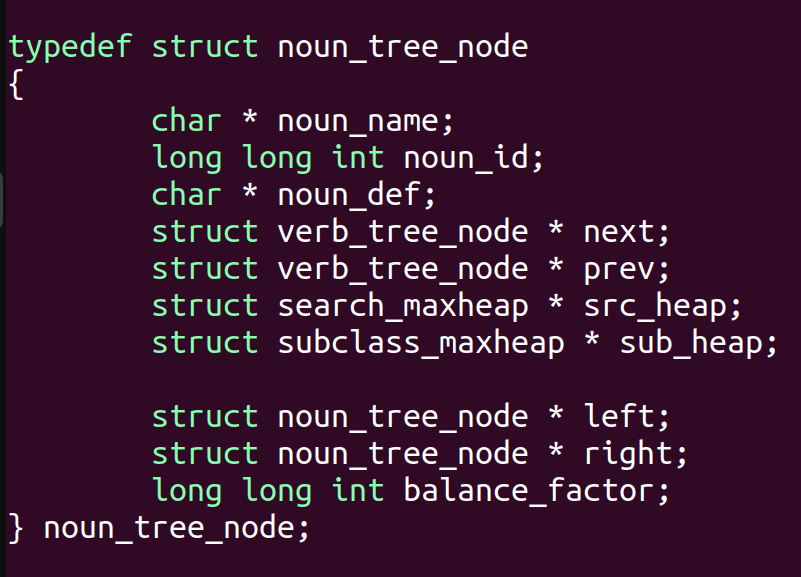
\includegraphics[width=0.8\linewidth]{c1.png} % Adjust the width as needed
\caption{Structural implementation in C}
\label{fig}
\end{figure}

AVL trees are used for their self-balancing property which ensures worst-case $O(\lg n)$ time complexity for search and insert operations.
Heaps, on the other hand, excel in extracting elements based on their priority with worst-case $O(\lg n)$ time complexity for insertion and retrieval. 


\subsection{Structure}

\subsubsection{Central Noun Tree}
The core of our knowledge graph is an AVL tree where each node represents a noun. Each noun node comprises the following elements:
    % 1. noun_name: A string representing the noun.
    % 2. noun_definition: A string containing the definition of the noun.
    % 3. noun_id: A unique identifier for the noun.
    % 4. prev_verb_tree: An AVL tree containing verbs that form backlinks to other nouns.
    % 5. next_verb_tree: An AVL tree containing verbs that form front links to other nouns.
    % 6. search_maxheap: A max-heap for extracting the highest priority connections.
    % 7. subclass_maxheap: A max-heap for accessing the highest priority subclasses of the noun.
\begin{itemize}

    \item \textit{noun\_name}: Pointer to a string representing the noun.
    \item \textit{noun\_id}: A unique identifier for the noun.
    \item \textit{noun\_definition}: Pointer to a string containing the definition of the noun.
    \item \textit{next\_verb\_tree}: An AVL tree containing verbs that form front links to other nouns.
    \item \textit{prev\_verb\_tree}: Pointer to an AVL tree containing verbs that form back-links to other nouns.
    \item \textit{search\_max-heap}: A max-heap for extracting the highest priority connections.
    \item \textit{subclass\_max-heap}: A max-heap for accessing the highest priority sub-classes of the noun.
    \item \textit{left, right, balance\_factor} : for maintaining AVL tree. 
    
\end{itemize}


\begin{figure}[htbp]
\centering
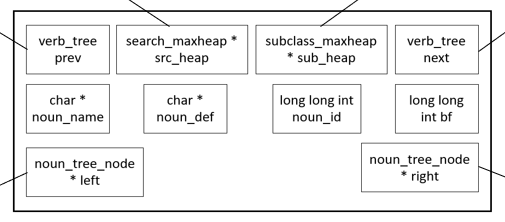
\includegraphics[width=0.8\linewidth]{fig_2_2.png} % Adjust the width as needed
\caption{Figure shows Structure diagram for Central Noun Tree node.}
\label{fig}
\end{figure}



\subsubsection{Verb Database Trees}
Two additional AVL trees are maintained to store:
\begin{itemize}
    \item verbs.
    \item verb descriptors.
\end{itemize}
These database trees serve as storage repositories to efficiently reuse allocated string memory. 
For example, if the verb "plays" occurs in multiple input lines, then memory for the string "plays" will be allocated only once and all the input lines will eventually point to the same memory ("plays").   
Nodes in these trees are not interconnected, focusing solely on memory optimization.

\\

\subsubsection{Sub-class Max\_heap}
This includes the sub-classes of the noun. For example, animal\_python,animal\_human and animal\_lion will be sub-classes of animal  
\begin{itemize}
    \item A pointer to the target noun node.
    \item \textit{weight}: The importance of the subclass.
\end{itemize}

\begin{figure}[htbp]
\centering
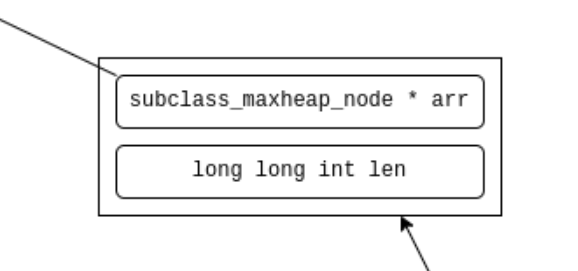
\includegraphics[width=0.8\linewidth]{subclass_maxheap.png} % Adjust the width as needed
\caption{Figure illustrates the Structure of Sub-class Max\_heap.}
\label{fig}
\end{figure}

\\

\subsubsection{Edge Representation}
Edges encapsulate the relationships between noun nodes. They are stored in the \textit{query\_max\_heap} of the verb nodes. Each edge contains:
\begin{itemize}

    \item \textit{noun\_ptr} : A pointer to the target noun node.
    \item \textit{truth\_bit}: A boolean indicating the truthfulness of the connection.
    \item \textit{end\_time}: The validity period of the connection.
    \item \textit{weight}: The significance of the connection.
\end{itemize}

\textit{Search\_maxheap} nodes point to these edges.
//




\begin{figure}[htbp]
\centerline{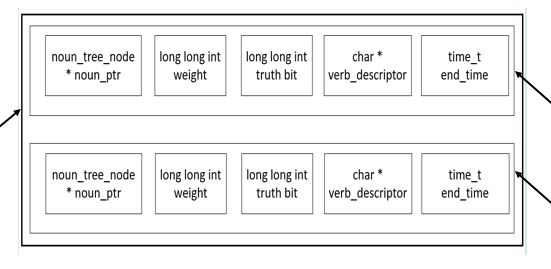
\includegraphics[width=0.5\textwidth]{fig_4_2.png}}
\caption{Figure illustrates the Structure of Edge.}
\label{fig}
\end{figure}



\subsection*{WorkFlow : Example of Entry Creation in the KG}

This section will illustrate how an entry is made in the KG.
For the input line : "Computer Science includes wide range of
Data Structures."

Here, the parser will identify "Computer Science" as "noun1" (1st noun of the sentence)
and "Data Structures" as "noun2" (2nd noun of the given input sentence).
Phrases like "includes" will be classified as "verb" and "wide range of" as "verb-descriptors".

Now there comes a need to store this sentence into the memory where our structural concept
of KG comes into use.
noun1 and noun2 (i.e., "Computer Science" and "Data Structures") will be inserted into the central AVL 
tree (explained in section ....) where all nouns are stored.

A new noun i.e., noun3 also gets formed: i.e., noun1 + "\_" + noun2 i.e., "Computer Science\_Data Structures"
and will be inserted in the central AVL tree (reason prescribed in section ...).

Each noun should only be inserted if it does not already exist in the central AVL tree. 
This prevents duplicates, ensuring no redundant nouns are stored, thus optimizing memory usage.

If the noun already exists, connections will be made through the existing noun itself.

The verb "includes" and verb descriptor "wide range of" are also stored in a similar manner
in the Verb Tree and Verb descriptor Tree (explained in section ....).

Further, irrespective of which branch of the central AVL tree the noun gets inserted, 
the connections among them are made, i.e.:

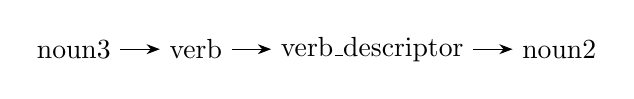
\begin{tikzpicture}[node distance=1.5cm, >=Stealth]
    \node (noun3) {noun3};
    \node (verb) [right=0.5cm of noun3] {verb};
    \node (verb_descriptor) [right=0.5cm of verb] {verb\_descriptor};
    \node (noun2) [right=0.5cm of verb_descriptor] {noun2};

    \draw[->] (noun3) -- (verb);
    \draw[->] (verb) -- (verb_descriptor);
    \draw[->] (verb_descriptor) -- (noun2);
\end{tikzpicture}

(explained in section ....)

In instances where the input line "Computer Science includes a wide range of Data Structures." is 
repeated, instead of creating new connections, the weights associated with the connections 
will be incremented, ensuring no redundant data and connections are stored.

This structure helps maintain the relationships within the knowledge graph, 
ensuring that each entry is efficiently organized and connected.


\subsection*{WORKFLOW: OUTPUT EXTRACTION FROM KG}

As an end-user, one may seek the most relevant response to their query. Users might ask questions such as:
\begin{itemize}
    \item "Computer Science includes?"
    \item "? includes Data Structures"
    \item "Computer Science includes Data Structures: True or False?"
    \item Or broader queries like: "Describe Computer Science" or "Computer Science?"
\end{itemize}

Queries may also contain spelling errors, requiring the system to provide the most relevant output and potentially prompt the user with a "Did you mean?" suggestion.
\\
For example, if a user inputs: "Comptr Science includes?" 
\\the system should prompt:
\\
"Did you mean: Computer Science includes?" 
\\
and proceed based on the user's response.
\\

As developers, it is crucial to handle all these types of queries efficiently. Therefore, we introduced functions in C, such as `display\_info\_lines()` and `print\_info\_lines()`, which are detailed in subsequent sections.
\\

Responding to questions like "Describe Computer Science" could overwhelm the user with an extensive amount of data, as the KG may contain thousands of entries related to Computer Science. \\
To manage this, the algorithm prompts the user with a follow-up question: "How many lines of information do you need?" If the user specifies 10 lines, the system will display the top 10 most important and weighted connections. 
\\
If the user requests "as many lines as possible," the system will display all connections in decreasing order of their weights, utilizing a max heap to efficiently manage this prioritization.





\section{Querying and Traversal}


The approach for traversing the KG is "Weight Proportional Breadth-First 
Traversal."

Our current KG framework is built utilizing structured data. 
User can shoot their desired queries in an interactive manner. 

Suppose the KG receives the input "Computer Science includes ?" and the user requests: "I want 10 lines of data."
In the KG, data is stored as depicted in the figure:





Although the KG may contain thousands of connections, for simplicity, let's assume it has 3 direct connections.

Given the limited number of lines to be displayed, the KG will prioritize the connections based on their weights using a max heap structure and will allocate ratios to the nouns of the next connections. In this case, the ratios are split as 
3:2:1 
because the weights of the connections are in the ratio 3:2:1 (i.e., Data Structures, Programming Language, Interesting). The allowed lines will be distributed to the next nodes in these proportions, and this process will continue recursively until all the requested lines have been displayed.

This recursive algorithm is called `display\_info\_lines()`.



\subsection{\textbf{display\_info\_lines}}

This function takes
\begin{itemize}
\item \textit{input\_noun} : A string whose connections are to be displayed
\item \textit{total\_lines} : The maximum number of lines to be printed. 
\end{itemize}
For worst-case analysis, we consider \textit{total\_lines} to be arbitrarily large, and in the context of the C Programming Language, we have considered it to be INT\_MAX.
\\

display\_info\_lines does:

1) Search for \textit{input\_noun} : Search for the noun in the noun tree of the KG. This search is done to find a 100\% matching string. As discussed above, this takes  $O(kn \lg n)$  time where 
\\k = string in the noun tree that has maximum length
\\n = number of nouns (noun nodes) in the noun tree.

If a perfect match isn't found, then another search is done, which gathers all nouns that are matching more than a certain threshold, and an array of choices is generated from this traversal
% This entire process also takes $O(kn \lg n)$ time.\\
\\
2) \textit{Display array of choices}: This is displayed as a "did you mean : " question, to correct spelling mistakes, in which the user is prompted with matching nouns. Depending on the user’s choice, the traversal is done.\\

If the user wants to traverse all the $k$ options, then the recursive function print\_info\_lines is called for each options.
\\
For example, if the user inputs: "Describe Computer Scien", the system will prompt with suggestions such as:
"Did you mean:
\begin{itemize}
    
    \begin{enumerate}
        \item Computer Science ?
        \item Computer Scientist ?
        \item Computer Science Theory ?"
    \end{enumerate}
    % \item and potentially several other suggestions.
    % \item The user can then choose to select one or multiple options from the provided suggestions and get the desired output.
\end{itemize}
and potentially several other suggestions.
The user can then choose to select one or multiple options from the provided suggestions and get the desired output.


\subsection{\textbf{print\_info\_lines}}
There are two cases in this function:

\begin{itemize}
    \item \textbf{Too Few Lines Allocated for Printing:}
    
    Here, the input noun has fewer relations than the lines allocated for it. Therefore, it will print all its relations, and the function will return. If \( k \) lines are to be printed and the noun has \( m \) connections in its search max heap, then in the worst case, it will cost:
    \[
    T(k, m) = O(k \log m) \quad \text{(1)}
    \]
    Note that \( k \leq m \).
    
    \item \textbf{There are Enough Connections to Traverse:}
    
    A traversal queue data structure is used for this purpose. All \( k \) connections of the noun are retrieved, and lines are allocated to them. This operation takes \( O(k) \) time. Later, constructing the queue takes:
    \[
    T(k) = O(k \log k) + O(k) \quad \text{(2)}
    \]
    This is overall \( O(k \log k) \).
    \\
    Note that \( k > m \).
    
    Once the traversal queue has been constructed, the function \texttt{print\_info\_lines} will be called for each node in the queue. If it occurs that all connections have been processed and the number of allocated lines has not been exhausted, then the algorithm enters the subclass max heap of the input noun. The same procedure is followed: line allocation, queue construction, and recursive function calls. The algorithm terminates when one of the following conditions is met:
    \begin{itemize}
        \item There are no remaining relations to print.
        \item The number of allocated lines to print is exhausted.
    \end{itemize}
    
    The KG is designed to ensure that the same relation is not traversed or printed more than once.
\end{itemize}


\\
% In the worst-case, every node in the KG will have a connection to the starting node of the breadth-first traversal, with the node connections arranged in a "linked list" fashion. For example, if the input sentences are structured as follows:
% \begin{itemize}
%     \item noun\_a verb1 noun\_b     ... noun3 = noun\_ab
%     \item noun\_ab verb2 noun\_c	... noun3 = noun\_abc
%     \item noun\_abc verb3 noun\_d   ... noun3 = noun\_abcd
%     \item . . . and so on
% \end{itemize}

% Here we see that if the traversal begins at noun1, then it can be connected with at the most $n/3$ nouns. Hence, the function \texttt{print\_info\_lines} is called $n/3$ times which is $O(n)$.
% \\The worst-case time complexity of \texttt{print\_info\_lines}, $T_p$, is
% \begin{equation}
% 	T(n) = O(n \lg n)
% \end{equation}


% where $n$ is the total number of nodes (nouns) in the graph. 
% \\
% Since \texttt{display\_info\_lines} calls this function and the time complexity is asymptotically the same, \texttt{display\_info\_lines} is also worst case $O(kn \lg n)$

% Typically, not all nodes of the graph are traversed, and the time required is often less!


\section{ANALYSIS OF ALGORITHMS}
\subsection{Insertion}
% Insertion involves parameters that affect the time complexity.
The parameters that affect the time complexity of Insertion are:
\begin{itemize}
    \item Input noun1 string size = $in_{n1}$
    \item Input noun2 string size = $in_{n2}$
    \item Input verb size = $in_{v}$
    \item Input verb desc size = $in_{vd}$
    \item Input definition size = $in_{def}$
\end{itemize}

Firstly, creation of noun3 is done, which is a concatenation operation, which is a linear time complexity operation
\\
\begin{equation}
	T_{\text{concat}}(in_{n1}, in_{n2}) = O(in_{n1} + in_{n2}) = O(n)
\end{equation}

Now, the nouns, verb, and verb descriptor are searched in the trees of the KG:
\begin{itemize}
    \item Number of nouns in the tree = $p$
    \item Maximum string length of noun in the tree = $k$
\end{itemize}
AVL search will need to traverse till the leaf nodes in the worst case. Each comparison is a string comparison and hence takes linear time:
\begin{equation}
	T_{\text{noun\_insertions}}(k, p) = O(k \lg p) = O(n \lg n)
\end{equation}

% Since all the trees are trees of strings (key is the string), overall

The time complexity of searching in all the trees(centralized noun AVL tree , database trees that include verb and verb descriptor tree) will be:
\begin{equation}
	T_{\text{total}}(n) = O(n \lg n)
\end{equation}

If the nouns or verbs are not present, then their insertion  will cost $O(n \lg n)$ time complexity in the worst case.
\\
Next, we check if the connection already exists. This involves a linear search in various max\_heaps:
\begin{equation}
	T_{\text{searching\_heaps}}(n) = O(n)
\end{equation}
\\
Insertion into various heaps must be done if the edge does not exist. \\Consider : size of the heap = $k$
\\then, insertion is done in $O(\lg k)$.
\\
\begin{equation}
	T_{\text{heap\_insertions}}(n) = O(\lg n)
\end{equation}







\section*{RESULT}
The graph constructed with the input data consistently produces accurate outputs.
\\
KG can infer new knowledge by applying logical reasoning over the existing data, supporting both direct and transitive inference. This capability is crucial for applications such as question answering, where the system needs to derive answers that are not explicitly stated but can be inferred from the available data.
\\
The algorithm is able to segregate the contexts from the data, and is able to give an accurate and reliable KG.
\\
On a 16-bit processor:
For small inputs (10,000 lines), the code constructed the graph in 1 second, and querying was much more faster.
The code took less than 20 minutes to construct a graph from 1,20,000 input lines 
The querying took about a millisecond to fetch the desired output effectively.

\section*{CONCLUSION}
The structure of the KG eventually created ensures that correct relations are given for suitable query. It yields 100\% accuracy.
\\
It is an effective implementation of the concept of KG
\\
The further goal is to create a KG from unstructured data with the help of NLP, making it more scalable, as illustrated in the image:

\\
\begin{figure}[htbp]
\centering
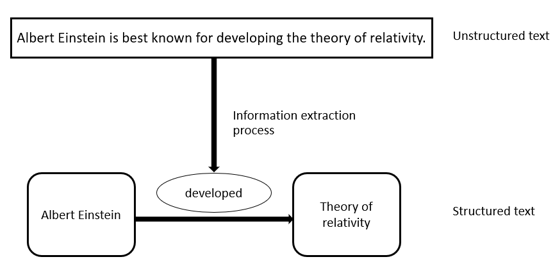
\includegraphics[width=0.8\linewidth]{nlp_img.png} % Adjust the width as needed
\caption{Figure illustrates the working of NLP}
\label{fig}
\end{figure}

% \section*{References}
\begin{thebibliography}{00}
\bibitem{b1} RDF Schema \url{https://www.w3.org/TR/2014/REC-rdf-schema-20140225/}
\bibitem{b2} Knowledge Graph for Products \url{http://dx.doi.org/10.1145/3336191.3371778}
\bibitem{b3} Arun Krishnan. 2018. Making search easier: How Amazon’s Product Graph is helping customers find products more easily. Amazon Blog. \url{https://blog.aboutamazon.com/innovation/making-search-easier}
\bibitem{b4} R. J. Pittman, Amit Srivastava, Sanjika Hewavitharana, Ajinkya Kale, and Saab Mansour. 2017. Cracking the Code on Conversational Commerce. eBay Blog. \url{https://www.ebayinc.com/stories/news/cracking-the-code-on-conversational-commerce/}
\bibitem{b5} Qi He, Bee-Chung Chen, and Deepak Agarwal. 2016. Building The LinkedIn Knowledge Graph. LinkedIn Blog. \url{https://engineering.linkedin.com/blog/2016/10/building-the-linkedin-knowledge-graph}
\bibitem{b6} Edgar Meij. 2019. Understanding News using the Bloomberg Knowledge Graph. Invited talk at the Big Data Innovators Gathering (TheWebConf). Slides at \url{https://speakerdeck.com/emeij/understanding-news-using-the-bloomberg-knowledge-graph}
\bibitem{b7} \url{https://medium.com/analytics-vidhya/introduction-to-knowledge-graphs-and-their-applications-fb5b12da2a8b}
\bibitem{b8} Aidan Hogan, Eva Blomqvist, Michael Cochez, Claudia D’amato, Gerard De Melo, Claudio Gutierrez, Sabrina Kirrane, José Emilio Labra Gayo, Roberto Navigli, Sebastian Neumaier, Axel-Cyrille Ngonga Ngomo, Axel Polleres, Sabbir M. Rashid, Anisa Rula, Lukas Schmelzeisen, Juan Sequeda, Steffen Staab, and Antoine Zimmermann. 2022. Knowledge graphs. ACM Computing Surveys. \url{https://arxiv.org/pdf/2003.02320}
\bibitem{b9} The C Programming Language \url{https://github.com/auspbro/ebook-c/blob/master/The.C.Programming.Language.2Nd.Ed%20Prentice.Hall.Brian.W.Kernighan.and.Dennis.M.Ritchie..pdf}
\bibitem{b10} SPARQL 1.1 Documentation \url{https://www.w3.org/TR/sparql11-query/}
\bibitem{b11} Neo4j Documentation 
\url{https://neo4j.com/docs/}
\bibitem{b12} Foundations of Modern Query Languages for Graph
Databases \url{https://dl.acm.org/doi/pdf/10.1145/3104031}
\bibitem{b13} RDF Data Storage and Query Processing Schemes \url{https://dl.acm.org/doi/pdf/10.1145/3177850}
\end{thebibliography}
\end{document}  
